\begin{minipage}[b]{0.6\textwidth}
\begin{Exercise}[label = circlemove, origin = J. Kaalda, title = Kreisbewegung, difficulty = 3]
	Wir betrachten zwei Kreisringe mit Radius $r$. 
%Einer der beiden ist in Ruhe, und der andere bewegt sich mit einer Geschwindigkeit $v$ so, dass die Mittelpunkte beider Kreise immer auf der gleichen Gerade liegen.\\
Einer ist in Ruhe, der andere bewegt sich mit der Geschwindigkeit $v$ entlang der Verbindungslinie beider Kreismittelpunkte auf ihn zu.\\ 
	Bestimme, wie die Geschwindigkeit des oberen Schnittpunkts der beiden Kreise, $P$, vom Abstand der Mittelpunkte, $d$, abhängt.
\end{Exercise}
\end{minipage}
\hfill
\begin{minipage}[b]{0.4\textwidth}
	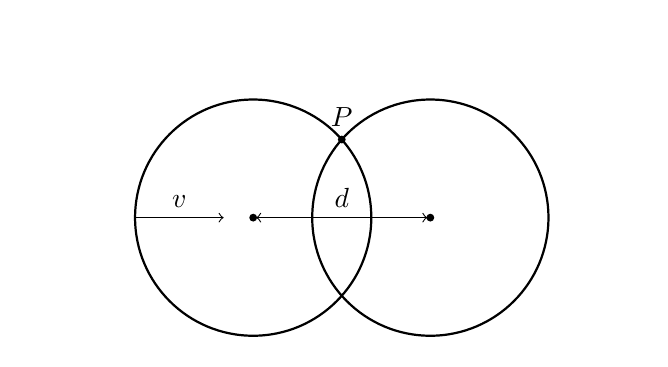
\begin{tikzpicture}[line cap=round,line join=round,x=1.0cm,y=1.0cm,scale =.75 ]
	\clip(-3.8185369414384267,-2.0485094372990885) rectangle (6.541366916798444,3.2167021331932286);
	\draw[thick](0.,0.) circle (2.cm);
	\draw[thick](3.,0.) circle (2.cm);
	\node [fill=black,inner sep=1pt,circle](a) at (3,0){};
	\node [fill=black,inner sep=1pt,circle](b) at (0,0){};
	\node[fill = black, inner sep = 1pt, circle]at (1.5,1.3228756555322954){};
%	\draw [<->] (3,0) to node[midway,above]{$d$} to (0,0);
	\node at (1.5,1.7) {$P$};
	\draw[->] (-2cm,0) to node[midway,above]{$v$} (-.5cm,0) ;
	\draw[<->](0.05,0) to node[midway,above]{$d$} (2.95,0);
	\end{tikzpicture}
\end{minipage}
\begin{Answer}[ref = circlemove]
	Bezeichne mit $\Gamma_1$ den ruhenden Kreis, und mit $\Gamma_2$ den sich bewegendenen Kreis.\\
	Die Lösung dieser Aufgabe kann sowohl elementargeometrisch, als auch in einem brachialen Analysisansatz gelöst werden.\\
	Elementargeometrisch geht das so:\\
	\begin{figure}[h]
		\definecolor{cqcqcq}{rgb}{0.7529411764705882,0.7529411764705882,0.7529411764705882}
		\centering
		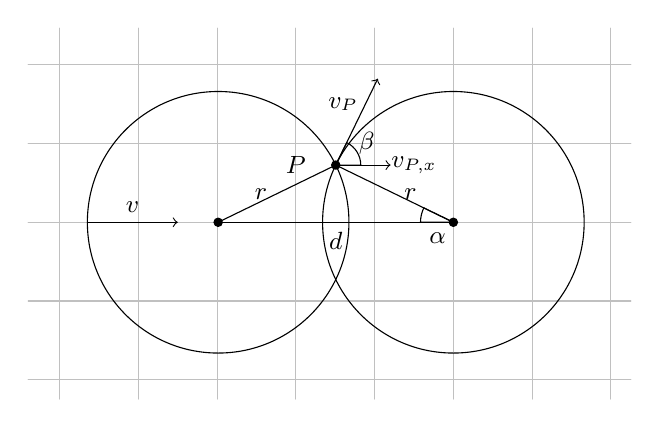
\begin{tikzpicture}[line cap=round,line join=round,x=1.0cm,y=1.0cm]
		\draw [color=cqcqcq, xstep=1cm,ystep=1cm] (-3.39930715163315,-2.2464251751178215) grid (4.25399001558093,2.4644111493984235);
		\clip(-3.39930715163315,-2.2464251751178215) rectangle (4.25399001558093,2.4644111493984235);
		\draw [shift={(2.,0.)}] (0,0) -- (154.06106822162783:0.41742321497767272) arc (154.06106822162783:180.:0.41742321497767272) -- cycle;
		\draw [shift={(0.5063907834922332,0.7265122637453222)}] (0,0) -- (0.:0.31742321497767272) arc (0.:64.06106822162783:0.31742321497767272) -- cycle;
		\draw(-0.9872184330155335,0.) circle (1.660930028932374cm);
		\draw(2.,0.) circle (1.660930028932374cm);
		\draw [->] (-2.6481484619479074,0.) to node[midway,above] {\small$v$} (-1.5,0.);
		\draw [->] (0.5063907834922332,0.7265122637453222) -- (1.039838521837773,1.8232073895930885);
		\draw (-0.9872184330155335,0.) to node[midway, left]{\small$r$}  (0.5063907834922332,0.7265122637453222);
		\draw (0.5063907834922332,0.7265122637453222) to node[midway,right]{\small$r$} (2.,0.);
		\draw (2.,0.) to node [midway, below] {\small$d$} (-0.9872184330155335,0.);
		\draw [->] (0.5063907834922332,0.7265122637453222) -- (1.2028175653942552,0.7265122637453222);
		\node at (.6,1.5) {\small$v_P$};
		\node at (1.8,-0.2) {\small$\alpha$};
		\node at (0.9,1) {\small $\beta$};
		\node at (1.5,0.7265122637453222) {\small$v_{P,x}$};
		\node at (0,0.7265122637453222) {\small $P$};
		\begin{scriptsize}
		\draw [fill=black] (-0.9872184330155335,0.) circle (1.5pt);
		\draw [fill=black] (2.,0.) circle (1.5pt);
		\draw [fill=black] (0.5063907834922332,0.7265122637453222) circle (1.5pt);
		\end{scriptsize}
		\end{tikzpicture}
	\end{figure}
	Wir können uns zuerst überlegen, wie groß die $x$-Komponente der Geschwindigkeit des Punktes $P$, $v_{P,x}$, ist. Dazu betrachten wir ein Bezugssystem, welches sich mit der Geschwindigkeit $\frac{v}{2}$ mitbewegt. In diesem ruht der Punkt $P$. Also ist $v_{P,x} = \frac{v}{2}$. \\
	Damit können wir $v_p$ ausrechnen. Es ist $v_p = \frac{v_{P,x}}{\cos \beta}$. Gleichzeitig ist $\beta = \frac{\pi}{2}-\alpha \Rightarrow v_p = \frac{v_{P,x}}{\sin{\alpha}}$.\\
	Der Winkel $\alpha$ ist aber durch das Dreieck zwischen $P$ und den beiden Kreismittelpunkten eindeutig bestimmt. Hier ist $\cos \alpha = \frac{d}{2r}$.\\	Wir können nun noch  $\sin\left(\arccos\left(x\right)\right)$ bestimmen. Hierfür hilft uns der trigonometrische Pythagoras, $\sin^2x + \cos^2x = 1$. Also ist
		$\sin\left(\arccos\left(x\right)\right) = \sqrt{1-	\cos^2\left(\arccos\left(x\right)\right)} = \sqrt{1-x^2}$.\\
	Damit ergibt sich für $v_p$
	\begin{align*}
		v_P &= \frac{v_{P,x}}{\sin\alpha} = \frac{v_{P,x}}{\sin\left(\arccos\left(\frac{d}{2r}\right)\right)}\\
		&= \frac{v}{2}\cdot \frac{1}{\sin\left(\arccos\left(\frac{d}{2r}\right)\right)}\\
		&= \frac{v}{2} \cdot \frac{1}{\sqrt{1-\frac{d^2}{4r^2}}}\\
		\Aboxed{&= \frac{v}{2} \cdot \sqrt{1+\frac{d^2}{4r^2-d^2}}.}
	\end{align*}

	
	
	Mit Analysis geht das so:
\begin{figure}[h]
	\centering
\definecolor{cqcqcq}{rgb}{0.7529411764705882,0.7529411764705882,0.7529411764705882}
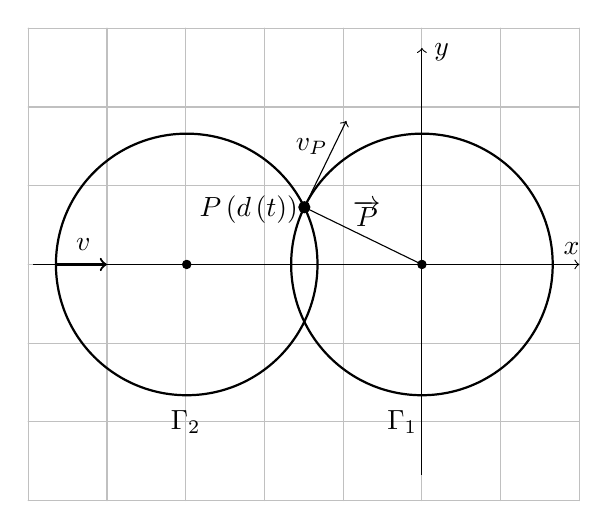
\begin{tikzpicture}[line cap=round,line join=round,x=1.0cm,y=1.0cm]
\draw [color=cqcqcq,, xstep=1.0cm,ystep=1.0cm] (-3,-3) grid (4,3);
\clip(-2.93679756017953,-2.665240279371838) rectangle (4.0099442229881435,2.9999474162114614);
\draw[thick](-0.9872184330155335,0.) circle (1.660930028932374cm);
\draw[thick](2.,0.) circle (1.660930028932374cm);
\draw [->, thick] (-2.6481484619479074,0.) -- (-2.,0.);
\draw [->] (0.5063907834922332,0.7265122637453222) -- (1.039838521837773,1.8232073895930885);
\node at (-.2,.7) {$P\left(d\left(t\right)\right)$};
\node at (-2.3,0.25) {$v$};
\node at (1.3,0.65) {$\overrightarrow{P}$};
\draw[->, thin] (2,-2.75) -- (2,2.75); 
\draw[->, thin] (-3,0) -- (4,0);
\node at (2.25,2.7) {$y$};
\node at (3.9,0.2) {$x$};
\node at (.6,1.5) {$v_P$};
\draw[] (2,0) -- (0.5063907834922332,0.7265122637453222);
\node at (-1,-2) {$\Gamma_2$};
\node at (1.75,-2) {$\Gamma_1$};
\begin{scriptsize}
\draw [fill=black] (-0.9872184330155335,0.) circle (1.5pt);
\draw [fill=black] (2.,0.) circle (1.5pt);
\draw [fill=black] (0.5063907834922332,0.7265122637453222) circle (2pt);
\end{scriptsize}
\end{tikzpicture}
\end{figure}\\
 Wir betrachten die Situation aus einem Koordinatensystem welches im Mittelpunkt von $\Gamma_1$ ruht.\\
	Die Punkte $\left(x_{\Gamma_1}, y_{\Gamma_1}\right)$ bzw. $\left(x_{\Gamma_2},y_{\Gamma_2}\right)$, die auf den Kreisen $\Gamma_1$ bzw. $\Gamma_2$ liegen, müssen nun die entsprechenden Kreisgleichungen erfüllen, die einfach nur besagen, dass auf dem Kreisumfang der Abstand zum Kreismittelpunkt konstant $r$ sein muss:
	\begin{equation}\label{circlemove:def}
		x_{\Gamma_1}^2 + y_{\Gamma_1}^2 = r^2 ~\mathrm{und}~\left(x_{\Gamma_2}+d\left(t\right)\right)^2+y_{\Gamma_2}^2 = r^2.
	\end{equation}
	Dabei definieren wir den Abstand, wie üblich, positiv, also $d\left(t\right) > 0$.\\
	Der Punkt $P$ soll nun auf beiden Kreisen liegen. Es gilt dann also $x_{\Gamma_1} = x_{\Gamma_2} =: x_p$ und $y_{\Gamma_1} = y_{\Gamma_2} =: y_p$. Die so entstehende Gleichung kann man jetzt gut nach $x_p$ auflösen:
	\begin{equation*}
		y_p^2 = r^2-x^2 = r^2-\left(x+d\right)
	\end{equation*}
	\begin{equation}\label{circlemove:xcoord}
		\Leftrightarrow 2xd + d^2 = 0 \Leftrightarrow x = \frac{-d}{2}.
	\end{equation}
	Das hätte man sich auch ander überlegen können.\\
	Wir betrachten jetzt den oberen Schnittpunkt. Das stellt keine Einschränkung da, weil seine Geschwindigkeit gleich der des unteren Punktes sein sollte.\\
	Dann gilt für die $y$-Koordinate $y_p$ des Punktes $P$
	\begin{equation}\label{circlemove:ycoord}
		y_P =  \sqrt{r^2-x_p^2} = \sqrt{r^2-\frac{d^2}{4}}.
	\end{equation}
	Damit können wir den Ortsvektor des Punktes $P$, $\overrightarrow{P}$, schreiben als
	\begin{equation}\label{circlemove:pvec}
		\overrightarrow{P} =\begin{pmatrix}
		x_p\\
		y_p
		\end{pmatrix}  = \begin{pmatrix}
		-\nicefrac{d}{2}\\
		\sqrt{r^2-\frac{d^2}{4}}
		\end{pmatrix}.
	\end{equation}
	Dabei ist hier $\overrightarrow{P}$ als Funktion von $d$ gegeben, $\overrightarrow{P}\left(d\right)$. Der Abstand $d$ ist aber selber nochmal eine Funktion der Zeit, $d = d\left(t\right)$.\\
	Die gesuchte Geschwindigkeit des Punktes $P$ ist jetzt der Betrag der (komponentenweise) Ableitung von $\overrightarrow{P}$ nach der Zeit, also $v_P = \left|\frac{d\overrightarrow{P}}{dt}\right|$. Mit der Kettenregel ergibt sich dann
	\begin{equation*}
		\frac{d\overrightarrow{P}}{dt} = \frac{d\overrightarrow{P}\left(d\right)}{dd}\cdot  \frac{dd\left(t\right)}{dt}.
	\end{equation*}
	Da gilt $\frac{dd\left(t\right)}{dt} = -v$ ergibt sich
	\begin{equation}
		\frac{d\overrightarrow{P}}{dt} = -v\cdot \frac{d\overrightarrow{P}\left(d\right)}{dd}.
	\end{equation}
	Wenn wir die Ableitung jetzt auswerten, kommen wir auf
	\begin{equation}\label{circlemove:pder}
		\frac{d\overrightarrow{P}}{dt} = v\cdot \begin{pmatrix}
		\nicefrac{1}{2}\\
		\frac{d}{2\sqrt{4r^2-d^2}}
		\end{pmatrix}.
	\end{equation}
	Den Betrag von $\frac{d\overrightarrow{P}}{dt}$ finden wir jetzt ganz einfach mit dem Satz des Pythagoras,
	\begin{equation}
	\boxed{
		v_p = \left|v\cdot \begin{pmatrix}
		\nicefrac{1}{2}\\
		\frac{d}{2\sqrt{4r^2-d^2}}
		\end{pmatrix}\right| = \frac{v}{2} \cdot \sqrt{1+\frac{d^2}{4r^2-d^2}}.}
	\end{equation}
	
\end{Answer}